\documentclass[
%===============================================================
%	DOCUMENT PREFERENCES
%===============================================================
	parskip		=	half,			% remove first-row indent in new paragraph
	headheight	= 	12pt,			% header height
	footheight 	= 	16pt,			% footer height
	headsepline,						% header separator line
	footsepline,						% footer separator line
	abstracton,						% Abstract headers
	headinclude	=	false,		
	footinclude	=	false,
	listof		=	totoc,			% List of ... in TOC
	toc			=	bibliography,	% Bibliography in TOC
	draft		=	false
]{scrreprt}

% Language and general symbol preferences
\usepackage[ngerman, english]{babel}
\usepackage[utf8]{inputenc}
\usepackage{soul}					% hyphening, etc.
\usepackage[super]{nth}				% superscript "n-th" (counting, etc.)
\usepackage{enumitem}
\usepackage{wasysym} 				% use additional symbols

% Page preferences
\usepackage[a4paper]{geometry}				
\geometry{
	a4paper,
	margin		=	2.5cm,
	foot 		= 	1.0cm
}

% Font preferences
\usepackage{couriers}
\KOMAoptions{fontsize=11pt}			% 12pt font size
\addtokomafont{disposition}			% Serif font for chapter headings
	{\rmfamily\bfseries}

\usepackage{setspace}				% 1.5x line spacing	
\onehalfspacing

% Header & Footer preferences
\usepackage{scrlayer-scrpage}		% Clear default settings
\pagestyle{scrheadings}
\clearpairofpagestyles

\ihead{Seminararbeit}				% Header left	(Type)
\automark{chapter}					% Header right	(Chapter)
\ohead{\rightmark}
\ifoot{DHBW Stuttgart}				% Footer left	(School)
\cfoot{Fuchs, Rudzinski}			% Footer center	(Author)
\ofoot[\pagemark]{\pagemark}			% Footer right	(Page mark)

%===============================================================
%	ADDITIONAL PREFERENCES
%===============================================================

% Bibliography preferences
\usepackage[style=ieee]{biblatex}
\bibliography{back-matter/literature.bib}

% Management packages
\usepackage[titles]{tocloft}			% ToC management
\setlength{\cftbeforechapskip}{5pt}
\setcounter{secnumdepth}{3}			% Sub-subsection numbering
\usepackage{array}					% Table management
\usepackage{multirow}
\usepackage{tabularx} 				% for breaking table entries

\usepackage{acronym}					% Acronym management
\usepackage{graphicx}				% Figure management
\usepackage{subfig}
\usepackage{hyperref}				% Referencing management
\hypersetup{}
\usepackage{inconsolata}			
	
% Misc
\setcounter{tocdepth}{2}				
\setcounter{lofdepth}{2}

%===============================================================
%	CUSTOM COMMANDS
%===============================================================

% Title page image handling
\newcommand*{\vcenteredhbox}[1]{
	\begingroup
	\setbox0=\hbox{#1}\parbox{\wd0}{\box0}
	\endgroup
}

% Remove page break on abstract
\newenvironment{absolutelynopagebreak}
{\par\nobreak\vfil\penalty0\vfilneg\vtop\bgroup}{\par\xdef\tpd{\the\prevdepth}\egroup\prevdepth=\tpd}

\usepackage{scalerel,amssymb}
\def\msquare{\mathord{\scalerel*{\Box}{gX}}}

%===========================================================================

\title{Fallstudie \textit{17A-Bank}: Architekturprozess} 
\author{Fionn Fuchs\\Oliver Rudzinski}
\date{12. Mai 2020}

%===========================================================================

\begin{document}
\makeatletter
\selectlanguage{ngerman}

%===========================================================================
%	FRONT MATTER
%===========================================================================

	\clearpage
	\hfill
\vcenteredhbox{
\includegraphics[height=2.5cm]{img/logo_dhbw.png}}

\vfill\vfill

\begin{center}
	\rule{\linewidth}{1pt}
	{
		\Huge \bfseries
			\@title
		\par	
	}
	\vspace{-0.2cm}
	\rule{\linewidth}{1pt}
	

	Seminararbeit (Aufgabe 7)
	\vfill
	
	für den Studiengang \\ \textbf{Informatik}
	
	an der \\ \textbf{Dualen Hochschule \\Baden-Württemberg\\Stuttgart}
	\vfill
	von \\ \textbf{\textsc{\@author}}
\end{center}

\vfill\vfill

\begin{tabbing}
	mmmmmmmmmmmmmmmmmmmmmmmm				\= \kill
	\textbf{Abgabedatum} \> \@date \\
	\textbf{Matrikelnummern} \> \texttt{9760520} (Fuchs)\\
	\> \texttt{5481330} (Rudzinski) \\
	\textbf{Modulbezeichnung} \> T3INF4322.1 \\
	\textbf{Unit} \> Architekturen von Businesssystemen \\
	\textbf{Kurs}	\> TINF17A \\
	\textbf{Dozent} \> Dr. Stefan Fütterling \\ 
\end{tabbing}
	\thispagestyle{empty}
	
	\pagenumbering{roman}
	
	\tableofcontents
	
%===========================================================================
%	MAIN MATTER
%===========================================================================
	
	\chapter{Einleitung}
		\pagenumbering{arabic}
		\label{chap:einleitung}
		Die 17A-Bank ist zur Zeit in vier Ländern aktiv (Deutschland, Slowenien, Tschechien und Österreich) und managt jedes davon unabhängig. Jedes Land hat dabei eine unabhängige IT-Infrastruktur, was sich als zunehmend problematisch gestaltet. Anwendungen und Daten liegen redundant und verstreut vor. In den vier Rechenzentren befindet sich ein Sammelsurium an Hard- und Software. Wartungsarbeiten können sich oft als komplex und teuer erweisen. Das alles führt nicht nur zu hohen Kosten, sondern macht es auch schwer bis unmöglich Daten zusammenzuführen um Beispielsweise ein Gesamtbild vom Kunden und seinem verhalten zu gewinnen. 

Zur Lösung dieser Probleme sollen die IT-Standorte und Rechenzentren zusammengeführt werden. Die vier Rechenzentren sollen dabei zu einem zentralen in Frankfurt konsolidiert werden. Die diversen Anwendungen für Girokonten, Sparkonten, Kredite und Kreditkarten sollen zukünftig auch konsolidiert werden. Aufgrund des hohen Aufwands einer Konsolidierung auf Anwendungsebene, hat sich die 17A-Bank für eine Konsolidierung auf Infrastrukturebene entschieden. Die Rechenzentren sollen also in ein modernes Rechenzentrum in Frankfurt zusammengelegt werden. Es sind bereits Standardplattformen für Storage und Server aufgebaut, sowie Standards für Betriebssysteme und Softwarestacks definiert. Das Rechenzentrum wird bei einem Hosting-Anbieter angemietet.

Um diesen Prozess sinnvoll und für die Mitarbeiter verständlich zu gestalten, sowie zukünftige Anwendungen besser in die bestehenden IT-Lösungen zu integrieren bedarf es eines Architekturprozesses.

Dieser soll eine Reihe von Anforderungen erfüllen:

Der Architekturprozess muss zunächst eine gute Zusammenarbeit zwischen Entwicklungsteams und Infrastrukturteams ermöglichen. Die Art und Weise, wie der Application Owner und die Entwicklungsteams über die Vorgaben der Architektur informiert werden und wie ihnen dabein geholfen wird diese umzusetzen und einzuhalten ist Teil der Architecture Governance (Kapitel 2.3). Infrastrukturarchitekten sollen frühzeitig in die Migrierungsprozesse involviert werden können. Gegebenenfalls soll er auch ein Deployment in eine Public Cloud ermöglichen. Er muss es ermöglichen die Anforderungen an Anwendungen flexibel zu definieren und umzusetzen.

Zusätzlich soll eine Checkliste für Application Owner, die in das neue Datacenter migrieren werden, ein Architecture-Governance Prozess und ein Genehmigungsprozess für Ausnahmen von der Architektur dargelegt werden.

	
	\chapter{Lösungserarbeitung}
		\section{Analyse: \textit{TOGAF} Architekturmethode}
	\label{sec:analyse}
	Der Prozess der Entstehung einer IT-Lösung beinhaltet verschiedene Schritte, Sichten und Abschnitte eines Unternehmens. Die erste Vision liefern hier meist Business-Consultants, indem diese sich auf die Businessanforderungen mit speziellen Fokus auf die gegenwärtigen Geschäftsprozesse berufen. Oftmals arbeiten diese mit Businessarchitekten zusammen. Im darauffolgenden Schritt folgt die Betrachtung der funktionalen Sicht mit Bezug auf die zu entwickelnde Anwendung, durchgeführt von Anwendungsarchitekten bzw. -entwicklern. Die Inbetriebnahme und praktische Durchführung geschieht im letzten Schritt bei der Betrachtung der operationalen Sicht, welche die nicht-funktionalen Anforderungen beschreibt. Diese Aufgabe wird von Infrastrukturarchitekten übernommen. Auch, wenn es sich hier um einen linearen Prozess handelt, muss die direkte Kommunikation und Zusammenarbeit zwischen zwei direkt aneinanderliegenden Aufgabenbereichen (und somit auch Enterprise-Architektenteams) unterstützt werden. Gerade bei der Migration bestehender Systeme sollten Infrastrukturarchitekten nicht aus dem Entwicklungsprozess herausgehalten werden \cite{Skript}.

Um eine gute Zusammenarbeit zwischen Entwicklungs- und Infrastrukturteams zu ermöglichen, um Infrastrukturarchitekturen frühzeitig in den Migationsporzess zu involvieren, bedarf es einer strukturierten Architekturmethode, welche die Kommunikation und Zusammenarbeit dieser beiden Parteien hervorhebt. Die folgenden Abschnitte analysieren, ob und wie sich das Architekturmodell TOGAF für diese Zielerreichung eignet.

\textit{The Open Ground Architecture Framework} (kurz TOGAF) liefert Ansätze für Entwurf, Planung, Implementierung sowie Instandhaltung von Enterprise-Architekturen. Die Entwicklung technischer Enterprise-Architekturen unterstützt TOGAF mit der sogenannten \textit{Architecture Development Method} (kurz ADM) \cite{TOGAFDocs}\cite{Matthes}\cite{VisualParadigmTOGAF}.

Die ADM empfiehlt eine Folge von neun Phasen für die technische Architekturentwicklung. Diese sind in der untenstehenden Abbildung dargestellt. Die Phasen A bis H sind hierbei zyklisch und gleichen sich iterativ mit sich und dem zentralen Requirements Management ab. Letzteres liefert eine dynamische Menge an unternehmensspezifischen Bedingungen und begleitet so den Entwicklungsprozess \cite{TOGAFDocs}. Abbildung \ref{fig:togaf_adm} veranschaulicht diesen Prozess.

\begin{figure}[h!]
	\centering
	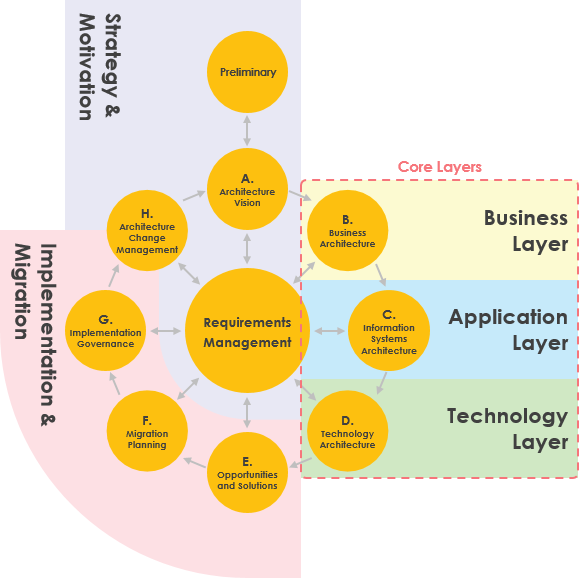
\includegraphics[width=0.8\linewidth]{img/togaf_adm}
	\caption{TOGAF ADM-Zyklus (nach \cite{VisualParadigmTOGAF})}
	\label{fig:togaf_adm}
\end{figure}

Wie zuvor beschrieben stellen die in der Grafik als \textit{Core Layers} bezeichneten Phasen den technischen Entstehungsprozess von IT-Lösungen dar. Die genannte Problematik der Kommunikation zwischen Anwendungs- und Infrastrukturentwicklern liegt hierbei in den Phasen C und D. Phase B wird in dieser Ausarbeitung aus Gründen der Aufgabenstellung vernachlässigt und daher als gegebener aber ebenfalls variabler Teil des Prozesses angesehen. Den Vorteil für die genannte Problematik bietet TOGAF ADM in der Art, wie jede einzelne Phase abgelaufen und wie diese dokumentiert wird \cite{Skript}\cite{TOGAFDocs}.

Jede Phase liefert einen definieren Output, basierend auf einen Input, welcher aus der Phase zuvor hervorgeht und durch phasengetreue Arbeitsschritte erweitert wird. Dieser Output wird auch als "Deliverable" bezeichnet. Während bestimmte Deliverables nur eine kurze Lebensdauer auf sehr begrenzte Phasenabschnitte aufweisen, werden zwei Output-Dokumente von Phase A bis F weitergereicht und be- bzw. überarbeitet. Dabei handelt es sich um das sog. \textit{Architecture Definition Document} (kurz ADD) und die \textit{Architecture Requirements Specification} (kurz ARS). Das ADD beinhaltet hierbei die Dokumentation der operationalen Modelle in unterschiedlichen Abstraktionsgraden und Darstellungsweisen. Die ARS hängt stark mit dem zentralen Requirements Management zusammen und beinhaltet nicht-funktionale Anforderungen unterschiedlicher Problembereiche (bspw. Anforderungen an das laufende System, an Änderungen an das System sowie etwaige Einschränkungen oder Gegebenheiten) \cite{Skript}. Da diese sowie durch die Anwendungsarchitektur (Phase C) sowie die Infrastrukturarchitektur (Phase D) geht, beinhaltet sie detailierte Ausarbeitung aus logischen als auch aus physischen Perspektiven. Diese Sichten betrachten jeweils zwei Zustände: Den Baseline- bzw. Ist-Zustand sowie den gewünschten Target- bzw. Soll-Zustand.  Dadurch sind beide Sichten und Zustände bei korrekter Anwendung des Modells optimal dokumentiert und können in Phase E evaluiert werden, wobei Phase F die Realisierung der Architektur vorsieht, an welcher Stelle die genannten Dokumente ADD und ARS finalisiert und freigegeben werden \cite{TOGAFDocs}\cite{VisualParadigmTOGAF}. Durch das Requirements Management können die jeweiligen Anforderungen von Anwendungs- und Infrastrukturteams ebenfalls frühzeitig erkannt und beachtet werden. Durch die interative Vorgehensweise erlaubt ADM ebenfalls die kontinuierliche, nachträgliche Verbesserung von getätigten Fehlentscheidungen, was ebenfalls vorteilhaft für den Zusammenhand zwischen Anwendungs- und Infrastrukturentwicklung ist. Dadurch ist es auch möglich, im Nachhinein getroffenen Entscheidungen reibungslos in den Prozess einzugliedern. Das könnte sich als vorteilhaft herausstellen, wenn die Architektur letztendlich in eine Public Cloud deployt werden soll.

Ungeachtet dessen beinhaltet ADM ebenfalls die Betrachtung der Implementation-Governance, welche in erster Linie keinen Bezug zur Anwendungs-Infrastruktur-Interdependenz aufweist, jedoch hilfreich und sinnvoll für die weitere Aufgabenstellung erscheint.

Zusammengefasst ist TOGAF ein geeignetes Modell für die gegenwärtigen Gegebenheiten, da es Anwendungsarchitekten und Infrastrukturarchitekten in ihrer Kommunikation unterstützt. Das geschieht über das iterative ADM mit zentralem Anforderungsmanagement sowie der vorteilhaften Dokumentation und Evaluation aller relevanten Sichten und Perspektiven der jeweiligen Beteiligten.

\section{Migrations-Checkliste für Application Owner}
	\label{sec:checkliste}
	Auch für die Migration auf die Soll-Architektur (oder auch \textit{Target Architecture}) sieht das ADM von TOGAF eine eigene Phase vor \cite{TOGAFDocs}. So stellt Phase F das Migration Planning dar und knüpfen somit direkt an die Evaluationsphase E "Opportunities and Solutions" an. Phase F sieht die Erstellung einer sog. Architecture Roadmap vor, welche die tatsächliche Implementierung unterstützt. Dieser Prozess versichert, dass die geplante Migration entsprechend der unternehmensspezifischen Vorgaben und Ziele durchgeführt wird, und dass die Faktoren Wert und Geld, welche im Rahmen dieser Aufgabestellung von großer Bedeutung sind, von allen Beteiligten nachvollzogen werden können \cite{VisualParadigmTOGAF}. Die Aufgabenstellung nimmt ebenfalls an, dass Entscheidungen rund um die Bestandteile und deren Realisierbarkeit bereits getroffen wurden, weswegen die Vorbereitungsschritte der Phase F hier vernachlässigt werden können.

Im Folgenden wird eine Reihe von Tätigkeiten für Application Owner nach TOGAF ADM vorgeschlagen, welche als Checkliste (s. Anhang \ref{app:checkliste}) für den praktischen Migrationsprozess genutzt werden können.

Da es sich oftmals um einen Migrationsplan handeln kann, welcher aus mehreren Teilschritten besteht, müssen diese Teilprojekte für die praktische Umsetzung priorisiert werden. Dazu erfolgen Bemessungen und Bewertungen der einzelnen Projekte nach unterschiedlichen Gesichtspunkten, u.a. kritischen Erfolgsfaktoren oder definierten Kriterien für Return on Investment.

Zwar sind die Zielressourcen definiert, jedoch ist die Verfügbarkeit und deren Implementierungsanforderungen eventuell nicht geklärt. Dies muss entsprechend geschehen und in die Priorisierung mit einfließen.

Ein weiteres Kriterium ist die Betrachtung der einzelnen Risikofaktoren der unterschiedlichen Teilprojekte, wobei sich dafür eine Szenariomethode eignen kann.

Mit diesen Eingaben und den entstehenden Prioritäten kann die besagte Architecture Roadmap angelegt und dokumentiert werden, welche die praktische Migration zeitlich und logistisch definiert.

Da TOGAF auch für nicht-technische Architekturen angewendet werden kann, sind die o.g. Punkte sehr abstrakt formuliert. Um die Priorisierung dennoch vollführen zu können, unterstützen folgende Fragestellungen über Komplexität und Dringlichkeit: Wie wurden die Anwendungen entwickelt, sind die Dokumentationen verfügbar und wie viele Unternehmensbereiche werden von der Migration beeinflusst? Darüber hinaus kann ebenfalls betrachtet werden, wie sehr der Unternehmenserfolg von der Anwendungsmigration abhängig ist und wie diese verwaltet wird.

Zusammengefasst können diese Schritte dazu verwendet werden, um einen prioritätsgetreuen Handlungsablauf zu planen, welcher die Migration des Systems auf sämtlichen Ebenen plant.

\section{Architecture Governance}
	\label{sec:governance}
	Die Architecture Governance ist dafür verantwortlich sicherzustellen, dass die Enterprise Architecture konsistent in allen Projekten eingehalten wird. Im Bezug auf das Datacenter und die darin laufenden Anwendungen bedeutet das kontinuierlich bestimmte Aspekte zu überwachen.

Entscheidende Aspekte die überwacht werden sollten sind Metriken, wie zB. die Auslastung des Datacenters oder einzelner Komponenten, sowie Anwendungsspezifische Metriken, die sich aus der Natur der Anwendung ergeben. Auch die Compliance der Anwendungen mit den Vorgaben und Richtlinien der Enterprise Architecture, sowie die Einhaltung von definierten Prozessen (zB. Migrierung) sollten kontinuierlich überwacht werden. Bei Veränderungen im Datacenter, beispielsweise durch Skalierung und Erweiterung sollte durch Beobachtung sichergestellt werden, dass diese mit den Businesszielen einhergehen. \cite{datacenter-architecture} 

Metriken können sehr hilfreich dabei sein Richtungen für Verbesserungen zu finden. Beispielsweise bei zu niedriger oder zu hoher Auslastung des Datacenters sollte über eine entsprechende Skalierung nachgedacht werden.

\begin{figure}
	\centering
	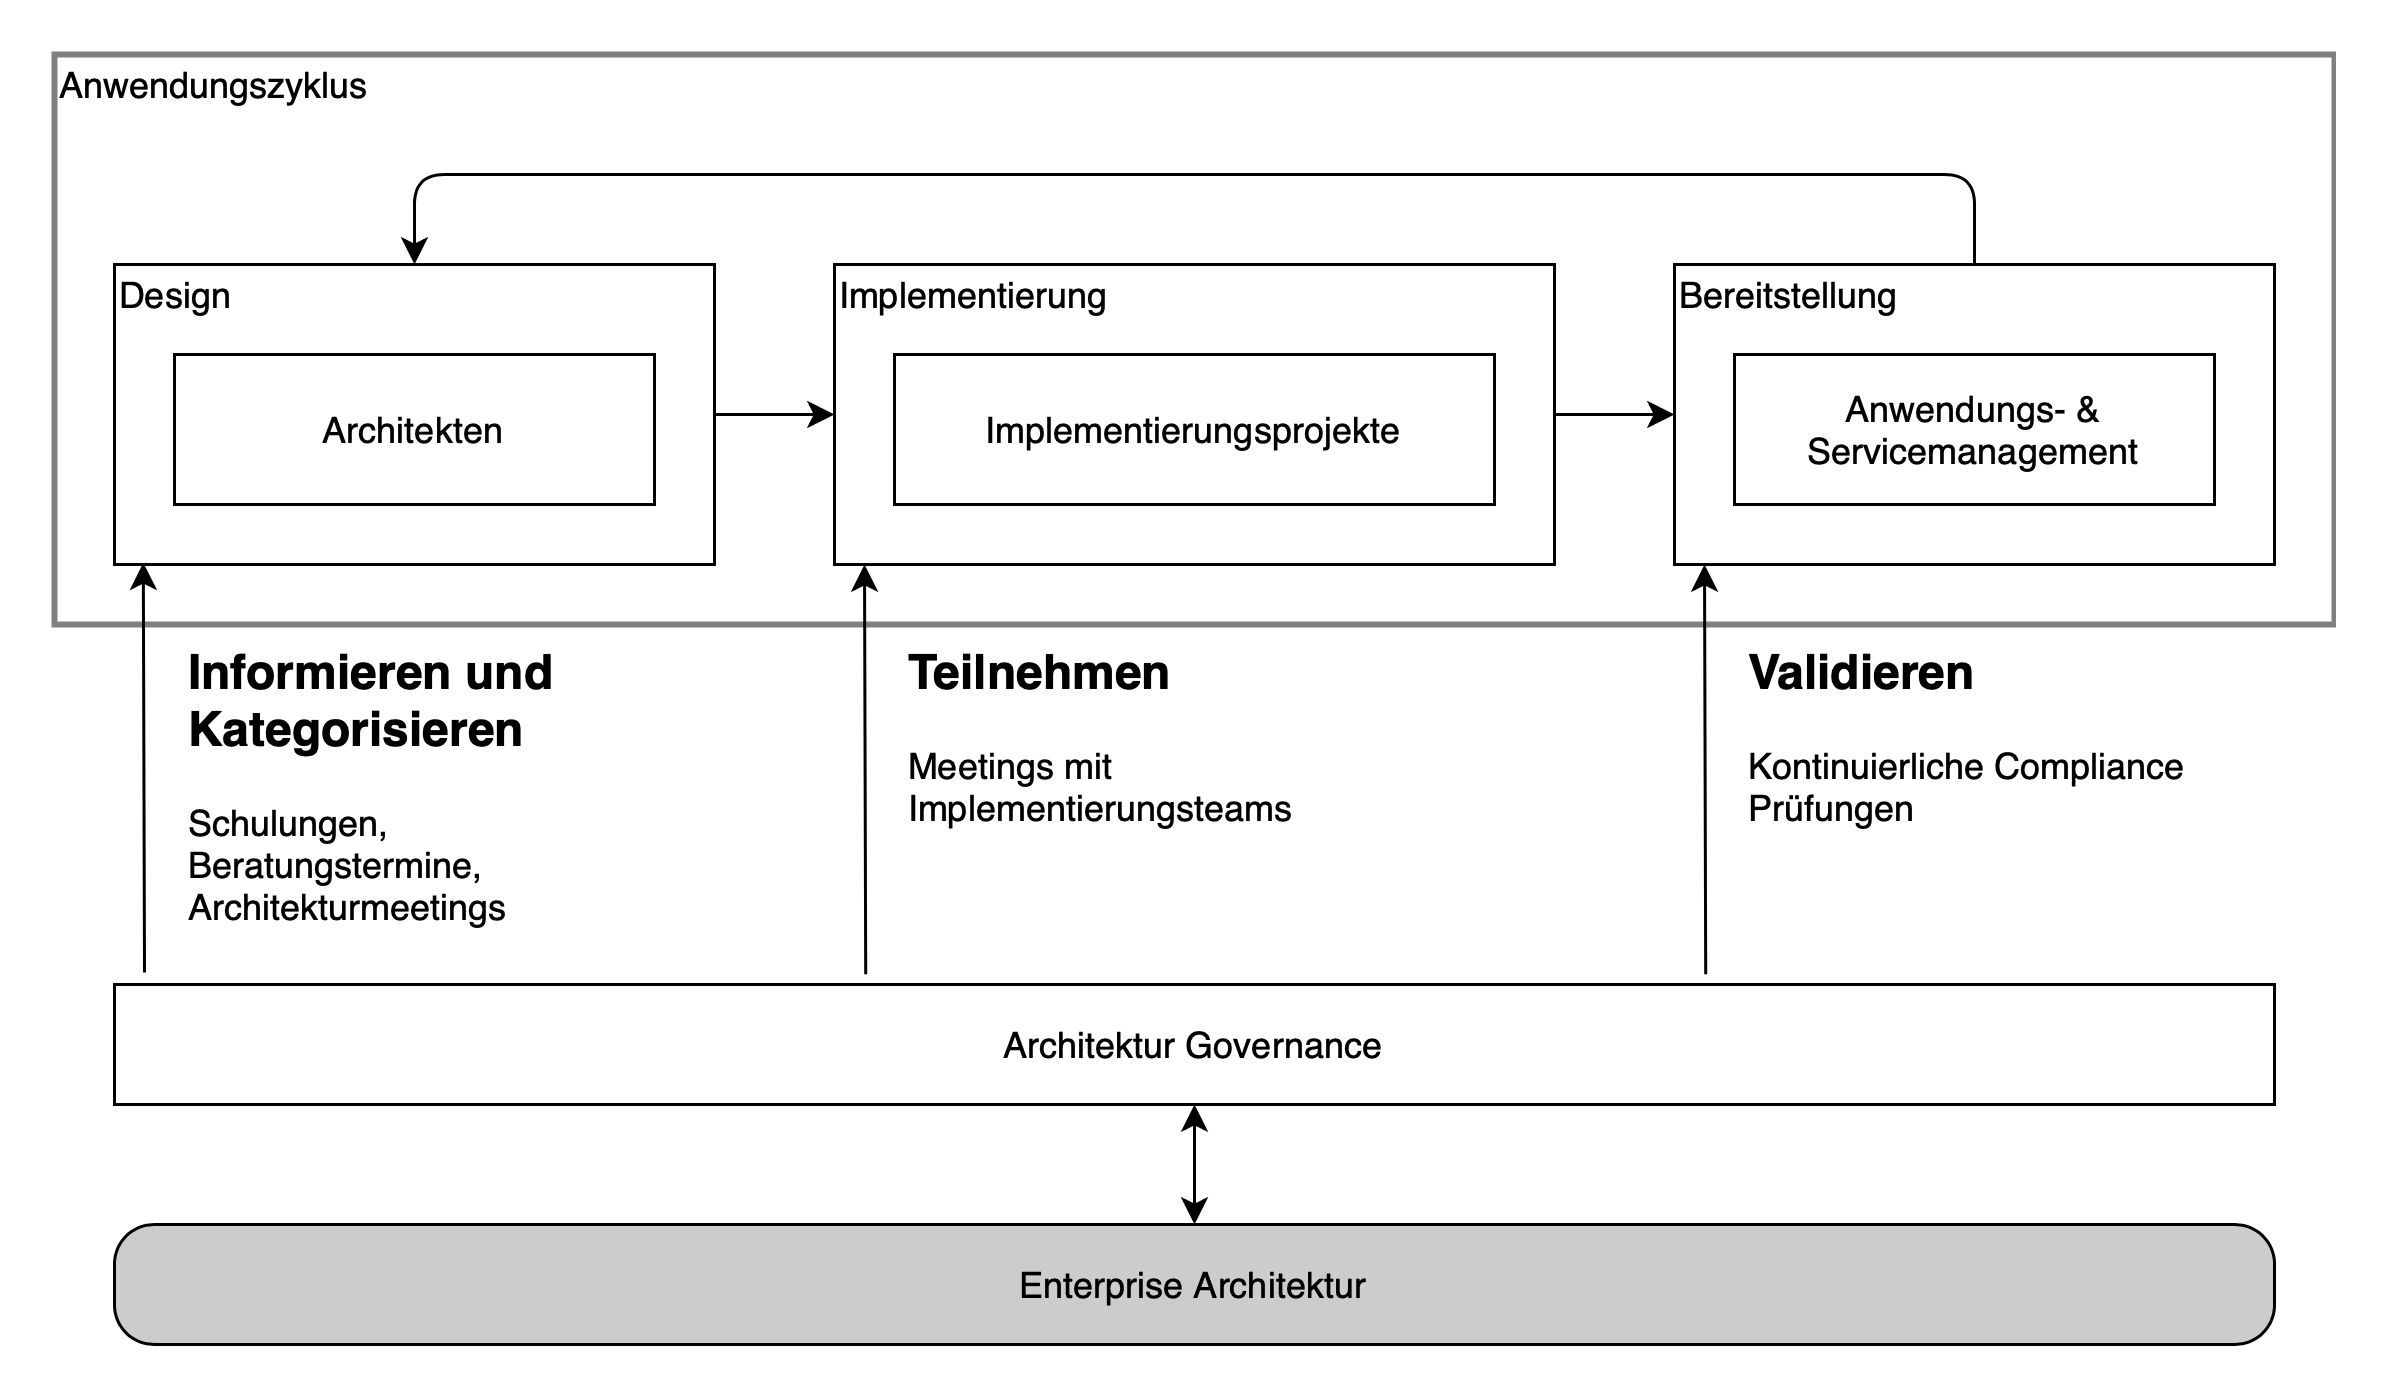
\includegraphics[width=\linewidth]{img/governance}
	\caption{Prozessübersicht der Architecture Governance}
	\label{fig:governance}
\end{figure}

Einer der wichtigsten Aufgaben der Architecture Governance ist es den Anwendungszyklus zu überwachen. Diese Aufgabe lässt sich in vier Teile unterteilen \cite{governance-approach}:

\begin{itemize}
	\item Informieren
	\item Projekte Kategorisieren
	\item An Entwicklung teilnehmen
	\item Validieren
\end{itemize}

Über die drei Phasen des Anwendungszyklus (Design, Implementierung, Bereitstellung) hinweg, ist die Architecture Governance konstant beteiligt. In der Designphase sollte es Angebote für Beratungstermine und Schulungen für Architekten geben, um sie mit der Enterprise Architecture vertraut zu machen und sie bei der Gestaltung der Anwendung in Übereinstimmung mit den Vorgaben zu unterstützen. In der Implementierungsphase sollte es fortlaufend Meetings mit den Implementierungsteams geben um sicherzustellen, dass die Anwendung nicht von den Vorgaben abweicht. In der Bereitstellugnsphase müssen bereitgestellte Anwendung kontinuierlich auf Compliance überprüft werden. Da die Bereitstellungsphase direkt zurück zur Designphase führt müssen eventuelle Änderungen der Architektur, die Änderungen an Anwendungen erforderlich machen sowohl hier, als auch in der Designphase kommuniziert werden. Auch müssen in der Bereitstellungsphase die Metriken der Anwendung überwacht werden.


\section{Vergabe von Ausnahmegenehmigungen}
	\label{sec:ausnahme}
	Wenn eine Anwendung die Anforderungen, die durch die Architektur gegeben sind noch nicht erfüllt, aber trotzdem zeitnah bereitgestellt werden muss, gibt es einen Prozess um eine eingeschränkte Ausnahmegenehmigung zu erhalten. Eine Anwendung kann solch eine Ausnahmegenehmigung erhalten, wenn durch technische Hürden aktuell keine Compliance erreicht werden kann, der Compliance Prozess eine Geschäftsentscheidende Anwendung aufhält, wodurch substantielle Verluste zu erwarten sind, oder wenn die Enterprise Architektur nicht auf die Anwendung anwendbar ist. 

Mindestens einer der genannten Fälle muss nach Prüfung des Einzelfalles zutreffend sein, damit eine Ausnahmegenehmigung erteilt wird. In allen Fällen muss die Anwendung den vollständigen Compliance Prozess jedoch zu einem späteren Zeitpunkt, der bei der Erteilung einer Ausnahmegenehmigung festesetzt wird, durchlaufen. 

Sollte sich bei der Prüfung des Antrags auf Ausnahmegenehmigung herausstellen, dass keiner der genannten Gründe erfüllt ist, muss ein Beratungstermin mit dem verantwortlichen Architekten oder Implementierungsteam stattfinden, der zur Aufklärung dient. Dies soll die Anzahl an nicht notwendigen Anträgen minimieren. 

Sollte sich bei der Prüfung herausstellen, dass die Enterprise Architektur nicht auf die Anwendung anwendbar ist, muss ein entsprechender Prozess zur Erweiterung oder Anpassung der Architektur angestossen werden und der Termin für Compliance Prüfung der entsprechenden Anwendung nach dem Abschluss dieses Prozesses stattfinden.

Für Ausnahmen von der Architektur wird ein 5-Phasen Modell vorgeschlagen \cite{exception-governance}:

\begin{enumerate}
\item Ausnahmezustand: Eine Ausnahme von der Architektur besteht
\item Gelöst: Die Ausnahme wurde beseitigt
\item Aufgelöst: Die Lösung der Ausnahme wurde vom Application Owner abgesegnet
\item Archiviert: Die Ausnahme bleibt für Dokumentationszwecke archiviert
\item Gelöscht: Die Ausnahme ist gelöscht und nicht länger in der Dokumentation aufzufinden
\end{enumerate}

Regel: Anwendungen dürfen, wenn überhaupt, nur temporär ohne erfolgreiche Compliance Prüfung bereitgestellt werden.

		
	\chapter{Einbettung des Lösungsvorschlages}
		Um die genannten Punkte des letzten Kapitels praktisch in die Tat umzusetzen, müssen bestimmte Vorbereitungen getroffen werden. Zunächst muss evaluiert werden, ob TOGAF als neue Architekturmethode für die bestehenden Teams zu der bestehenden Zeit der Migration überhaupt in Frage kommt. Faktoren, die für diese Evaluation eine Rolle spielen, sind u.a. der jetzige Stand der Migration, die Bereitschaft der Mitarbeiter einer grundlegenden Arbeitsanpassung, sowie der geschätzte Aufwand, bestehende Prozesse auf TOGAF umzustrukturieren. Stellt sich heraus, dass die Umstrukturierung realisierbar und sinnvoll ist, müssten Schulungen der Mitarbeiter und eben genannte Prozessveränderungen getätigt werden, bevor die Arbeit am eigentlichen Projekt wieder aufgenommen werden kann. Die benötigten Dokumentationen müssten ebenfalls nachträglich angelegt werden, um nahtlos innerhalb der Prozesses an die folgenden Schritte anknüpfen zu können. Sofern diese Fragestellungen geklärt sind, bedarf die praktische Umsetzung der Architecture Governance in jedem Fall die Absprache mit der Rechtsabteilung der Bank, vor allem mit Betrachtung auf die definierte Regelung der Ausnahmegenehmigungen. 
		
	\chapter{Zusammenfassung und Ausblick}
		Die 17A-Bank braucht zur erfolgreichen Umsetzung ihres neuen Datacenters einen fähigen Architekturprozess. Dafür eignet sich TOGAF als Methode zur Entwicklung einer Architektur. Um Anwendungen erfolgreich in das neue Datacenter zu migrieren wurde eine Checkliste für Application Owner entwickelt. Diese ist auch in kompakter Form im Anhang zu finden. Die Architecture Governance muss den Implementationsprozess neuer Anwendungen beobachten und entsprechend vorgeschlagene Maßnahmen treffen um Übereinstimmung mit Richtlinien der Architektur zu gewährleisten. Eingeschränkte Ausnahmegenehmigungen um Anwendungen temporär ohne Übereinstimmung mit der Architektur bereitzustellen sind unter besonderen Umständen möglich. Die 17A-Bank hat nun die Mittel eine sinnvolle Architektur zu gestalten.
	
%===========================================================================
%	BACK MATTER
%===========================================================================

	\clearpage
	\pagestyle{plain}
	\pagenumbering{alph}
	\printbibliography
	
	\appendix
		\pagestyle{plain}
		\chapter{Migrations-Checkliste}
	\label{app:checkliste}
	
\begin{itemize}
	\item[$\msquare$] Migrationsprojekt in Unterprojekte aufteilen
	\item[$\msquare$] Initialfragen für Unterprojekte klären
	\begin{itemize}
		\item[$\msquare$] Wie wurde die Anwendung entwickelt?
		\item[$\msquare$] Ist die Dokumentation der Anwendung verfügbar?
		\item[$\msquare$] Wie viele Unternehmensbereiche sind direkt durch die Prozesse der Migration betroffen?
		\item[$\msquare$] Wie stark hängt der Unternehmenserfolg von dem Unterprojekt ab?
		\item[$\msquare$] Wie wurde die Anwendung verwaltet?
	\end{itemize}
	\item[$\msquare$] Bemessung der Prioritäten
	\begin{itemize}
		\item[$\msquare$] kritische Erfolgsfaktoren
		\item[$\msquare$] Return on Investment?
		\item[$\msquare$] ...
	\end{itemize}
	\item[$\msquare$] Risikoanalyse der Unterprojekte (Szenarioanalyse)
	\item[$\msquare$] ggf. Anpassung der Prioritäten
	\item[$\msquare$] Aufstellen der Migrations-Roadmap (zeitlich sowie räumlich, priorisierte Unterprojekte zu Anfang)
\end{itemize}

	
	
\end{document}